\chapter{A multi-view modeling framework\label{chapter:framework}}

This chapter installs the necessary background about the formalisms we use and sets up our multi-view modeling framework. That is, we've decided to present the technical background \emph{in situ}. Indeed, strictly speaking, the multi-view framework is a contribution of this thesis, but almost all its technical pieces -- formalisms, algorithms and techniques -- are not. Presenting them together, however, allows us to explain and reconcile two related but different visions of model synthesis.

The framework is illustrated in Fig. \ref{image:framework}, that also provides a key for reading this chapter. As shown, the semantics of our models is grounded on classical \emph{trace theory}~\cite{Hoare:1985}. A \emph{trace} is a finite sequence of symbols, a simple abstraction commonly used to capture the notion of ``observable behavior'' in the context of concurrent systems. In our case, the notion of behavior actually denotes interactions among agents forming a system, modeled as \emph{events} sent and received by agents in a synchronous fashion. A (possibly infinite) set of traces, also called a \emph{language}, is typically captured with a kind of automaton named a labeled transition system (LTS).

This trace-based setting is complemented with \emph{fluents}, that capture state-based propositions in terms of the occurrence of events. Among others, fluents provide a friendly interface between event-based models (e.g. scenarios and state machines) and state-based models (e.g. goals and domain properties). This mix of event-based and state-based abstractions provide a precise meaning, consistent \emph{semantics}, to all models used in this thesis. 

\begin{figure}[t]\centering
  \scalebox{0.55}{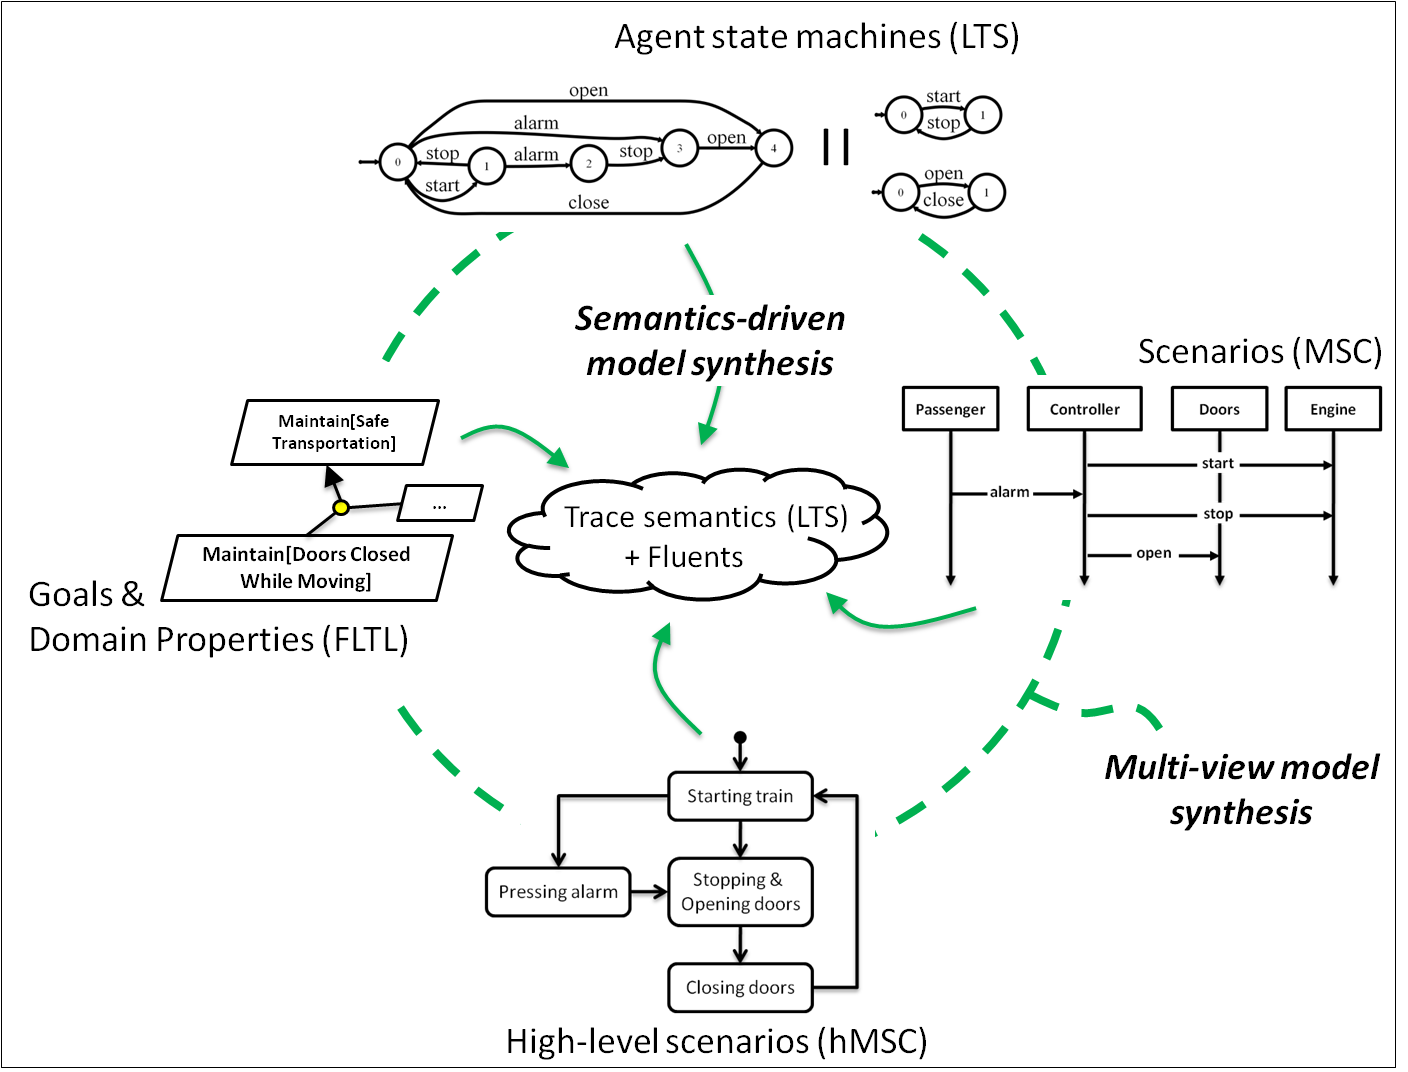
\includegraphics[trim=2mm 2mm 2mm 2mm, clip]{src/2-framework/images/framework}}
  \caption{Semantics and Multi-View consistency in our formal framework.\label{image:framework}}
\end{figure}

Observe however that LTSs are used in two different ways in this framework. On one hand, they provide a finite (and concrete) representation of infinite (and more abstract) sets of traces used to define the semantics of other models. On the other hand, they are incidentally chosen as a particular representation for agent and system state machines (even if one could argue that such a representation is too low-level to be of any practical use for end-users). 

We stress this distinction here because, to our opinion, it explains the differences between two different, yet complementary, usages of models and their synthesis. In some approaches, so-called ``low-level models'' are used to define the semantics or help analyzing other, higher-level models. In this case, the former are used either theoretically as pure mathematical objects or, technically, as synthesized artifacts used as input for model checkers, animators, etc. Whatever the case, low-level models are commonly kept hidden to the end-user, in contrast to the higher-level ones which are used as input language for her (see, e.g.,~\cite{Magee:1997, Uchitel:2003, Damas:2009}). This contrasts with other approaches where different kinds of models are considered on an equal footing to form a consistent, multi-view representation of a system. In this second case, model synthesis aims at enriching the model basis by generating missing models, or completing existing ones. Therefore, synthesized models are visible to the end-user, who is expected to understand their intended meaning in a precise way (see, e.g.,~\cite{VanLamsweerde:1998, Whittle:2000, Uchitel:2004, Damas:2005}).

These two settings are complementary. Indeed, providing automated support to the second, multi-view modeling approach, requires models to be grounded on a shared formal framework. This triggers for a mathematical characterization of their semantics and associated synthesis techniques. Also, a multi-view modeling approach triggers for the definition of rules governing the consistent usage of multiple models. These rules are expressed in terms of the formal model semantics, even if different from the latter \emph{per se}. Synthesis-driven semantics is both used \emph{against} inter-model consistency rules, to verify them or prove their violation through a counter example (model-checking is worth noting here) and \emph{towards} them by synthesizing missing model views in a ``correct by construction'' fashion (see chapter~\ref{chapter:inductive-synthesis} for example).

The rest of this chapter is organized as follows. After a short description of our running example in the next section, Section~\ref{XX} provides background on trace semantics and labeled transition systems. Section~\ref{XX} then explains how the latter can be used as simple state machines to model agent behaviors and their composition. The trace semantics of scenarios and how they fit with state machines is detailed in section~\ref{XX}. We then turn to state based abstractions by describing fluents and their use in state invariants in Section~\ref{XX}, and goals and domain properties in Section~\ref{XX}. We close this chapter with a discussion in Section~\ref{XX}. 

\section{Running example: A toy train system}

We use a simple train system fragment as running example for illustrating concepts and techniques throughout this thesis. The system is composed of an automated train controller, actuators for doors and the engine as well as the latter themselves, sensors, and a passenger. Via the actuators, the controller typically controls operations like starting or stopping the train, opening or closing the doors, and so on. A safety goal requires train doors to remain closed while the train is moving. If the train is not moving and the passenger presses the alarm button, the controller must open the doors immediately. If the train is moving and the passenger presses the alarm button, then the controller must stop the train first and then open the doors. Typical agent interactions for the latter case are depicted in Fig.~\ref{image:train-scenario-all-agents}. The precise semantics of such a scenario is made clear in the following sections.

\begin{figure}[H]\centering
\scalebox{0.75}{
  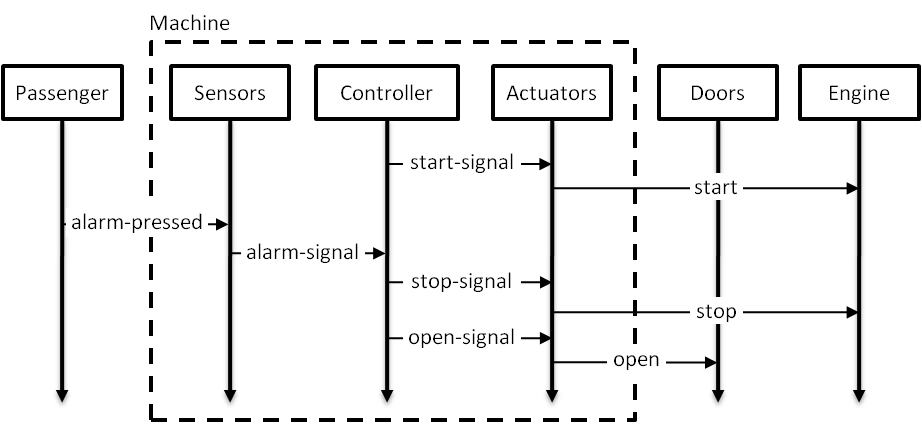
\includegraphics[trim=2mm 2mm 2mm 2mm, clip]{src/2-framework/images/train-scenario-all-agents}
}
\caption{A scenario illustrating a train system stopping in emergency when an alarm is pressed.\label{image:train-scenario-all-agents}}
\end{figure}


\section{Agents, System and their Behavior\label{section:background-agents-system-behaviors}}

A system is commonly admitted to be made of active components, called \emph{agents}, that behave and interact so as to fulfill system goals while restricting their behavior to ensure constraints they are assigned to~\cite{Feather:1987}. Some of them are human agents (the passenger), others are physical or electronic devices (e.g. the doors, the actuators), still others are software components (the automated controller). In addition to the notion of \emph{system}, that encompass all agents, the literature makes use of specific terms to distinguish between certain agents and/or agent aggregations. In~\cite{VanLamsweerde:2009} for example, the \emph{software-to-be} denotes software agent(s) that need to be developed (the automated controller, for example), while other agents compose its \emph{environment}. Another boundary consists in distinguishing the software together with its input and output devices from other agents. This boundary, depicted with a dashed line in Fig.~\ref{image:train-scenario-all-agents}, corresponds to the distinction made by Jackson between the \emph{world} and the \emph{machine}~\cite{Jackson:1995}. In this thesis, we focus on the behavior of a single agent as observed by the other agents with which it interacts (as opposed to its internal implementation). From the former agent perspective, then, the \emph{environment} is made of all these latter agents. 

In the light of the previous paragraph, we clearly need tools to capture single agent behaviors while being able to play with agent boundaries in a flexible manner -- for instance, for ``computing'' the behavior of agent aggregations like the \emph{software environment}, the \emph{machine} or simply, the \emph{system}. For this, we choose to model behaviors and interactions in an event-based framework, where agents communicate via messages that are sent and received simultaneously. Such kind of communication, called \emph{synchronous communication} or simply, \emph{message passing}, is motivated by its simplicity, an important aspect for accessibility to stakeholders involved during the early-design phase of a system. The next section introduces  labeled transition systems (LTS), the kind of model we use to capture agent behaviors. The next one presents operators for composing (and decomposing) them under a \emph{synchronous communication} hypothesis, a manner of capturing the behaviors of multiple interacting agents.

\subsection{Agents as Labeled Transition Systems}

In our framework, the behavior of an agent, say \artifact{Ag}, is modeled by a specific kind of finite state machine, called \emph{labeled transition system} (LTS). This formalism, initially introduced by Keller for reasoning about parallel programs~\cite{Keller:1976}, has since been intensively used for specifying and analyzing concurrent systems, e.g. in~\cite{Milner:1989, Clarke:1989, Magee:1997}. A LTS is made of a set of states and a set of transitions between them (see Fig.~\ref{image:framework-start-stop}). Each transition is depicted with an \emph{event} label -- sometimes called an \emph{action} label; also, a specific state is the \emph{initial state}, designated graphically by an empty arrow in front of it (state 0 in the figure). 

\vspace{0.5cm}
\begin{figure}[H]
\centering\scalebox{0.60}{
  \includegraphics*[clip]{src/2-framework/images/start-stop}}
  \caption{A Labeled Transition System for an \artifact{Engine} agent\label{image:framework-start-stop}.}
\end{figure}

Labeled transition systems come with different flavors in the literature that allows capturing more or less meaning, also resulting in few or numerous semantics subtleties. We stick here with a very simple framework, by restricting our attention to \emph{determinate} agents~\cite{Engelfriet:1985}, that is, agents whose behavior can be modeled using \emph{deterministic} transition systems (see below). While a somewhat restrictive choice in terms of expressiveness --~many approaches arising from process algebra do not restrict to such an hypothesis~-- we argue that it naturally keeps the framework simple and intuitive to use for stakeholders. We now turn to some mathematical definitions that, among others, define the aforementioned terms.

Mathematically, a LTS is defined as a 4-tuple $(Q,\Sigma,\delta,q_{init})$ where $Q$ is a finite set of states, $\Sigma$ is a set of labels called its \emph{alphabet}, $\delta$ is a transition relation $Q \times \Sigma\cup\{\tau\} \times Q$ and $q_{init} \in Q$ is the initial state.

A \emph{deterministic} LTS does not have $\tau$ transitions and has no state with two outgoing transitions having the same label (that is, $(q,l,q_1) \in \delta \wedge (q,l,q_2) \in \delta \implies q_1 = q_2$); otherwise it is \emph{non-deterministic}.

A \emph{terminating} state is one with no outgoing transition; otherwise it is \emph{non-terminating}. A \emph{terminating} LTS has at least one terminating state; otherwise it is \emph{non-terminating}. Note that, as such, the LTS definition does not allow distinguishing between terminating states that model successful termination -- an agent stops running intentionally -- and non-successful termination -- an agent, more often the system as a \emph{composed} agent (see next section), \emph{deadlocks} unintentionally. We will come back to this discussion in section~\ref{section:background-discussion}.

The \emph{alphabet} $\Sigma$ captures the notion of \emph{agent interface}, as a set of event labels that an agent recognizes or, said otherwise, in which the agent \emph{engages} in synchronous communications with its environment. For example, the LTS of Fig.~\ref{image:framework-start-stop} has an alphabet \artifact{$\Sigma=\{start, stop\}$}. Note that labeled transition systems do not distinguish between \emph{sent} and \emph{received} events. This distinction being required when playing with scenarios, we assume that an event label uniquely determines the interacting agents and that this architectural information is available elsewhere (typically, from the scenarios themselves). However, we allow an event label to be shared between more than two agents, but assume that only one of them is the \emph{sender}. By simplicity in the sequel, we denote $\Sigma\cup\{\tau\}$ by $\Sigma_{\tau}$ (an alphabet augmented with the $\tau$ label).

An finite LTS \emph{execution} is a finite sequence of its states separated by labels, i.e. \artifact{$w = \textless q_0,l_0,\ldots,q_{n-1},l_{n-1},q_n \textgreater$} with $q_i \in Q$ and $l_i \in \Sigma_{\tau}$. An execution is valid for a LTS if it denotes an existing path, from the initial state, in the corresponding graph; mathematically, $q_0 = q_{init}$ and $(q_i,l_i,q_{i+1}) \in \delta$ for $0 \leq i < n$. The projection of an execution $w$ over an alphabet $\Sigma$ is denoted by $w|_{\Sigma}$ and is the result of keeping, from $w$, only event labels that belong to $\Sigma$ (in other words, eliminating $q_i$ states and $\tau$ labels). Such a projection is also called a \emph{trace}, that we define now.

A \emph{trace} denotes an element of $\Sigma^*$, that is a finite sequence of event labels \artifact{$t= \textless l_0,\ldots,l_{n} \textgreater$} with $l_i \in \Sigma$. Unlike an execution, a trace never contains $\tau$ labels. A trace $t$ is accepted by a LTS if there exists a valid execution $w$ such that $w|_{\Sigma} = t$. In other words, a trace is \emph{accepted} by a LTS if it denotes an existing path in the corresponding graph from the initial path, but allowing ``in the middle'' silent moves offered by $\tau$ transitions in the non-deterministic case (and hence, possibly, more than one path). Note that, by this definition, a prefix of an accepted trace is also an accepted trace; the empty trace $\lambda$ is therefore always accepted. For example, the LTS of Fig.~\ref{image:framework-start-stop} accepts the trace \artifact{<start stop start>}, and hence \artifact{<start stop>}, but not \artifact{<start start>}. We sometimes use a dot notation $w.l$ to denote the concatenation of a trace $w$ with a label or another trace $l$.

The (maybe infinite) set of traces accepted by a LTS, say $P$, is called its \emph{language} and denoted by $\mathcal{L}(P)$. We naturally extend this notion to the language of an agent. For example, the  \emph{language} of the \artifact{Engine} agent is $\mathcal{L}(\artifact{Engine})=\{\lambda$, \artifact{<start>}, \artifact{<start stop>}, \artifact{<start stop start>}, \ldots $\}$. Actually, as prefixes of accepted traces are also accepted traces, LTS capture the class of \emph{prefix-closed} languages, a subclass of \emph{regular} languages~\cite{Hopcroft:1979}. This result opens the way of applying regular learning for synthesizing LTS, as detailed in chapter~\ref{chapter:inductive-synthesis}.

However, another important notion is the one of LTS \emph{equivalence} that permits answering questions like ``\emph{are agents $Ag_1$ and $Ag_2$ the same in term of their behavior?}''. Many different notions of behavioral equivalence exist in the literature, like \emph{strong} and \emph{observational}  equivalences~\cite{Milner:1989}. Their introduction (in process algebra) is motivated by the need to distinguish between particular process cases as well as being able reason about their correctness (in terms of \emph{deadlock}, for instance), especially when dealing with non-determinism. For details, see e.g.~\cite[chap. 3]{Hoare:1985}, \cite[chap. 4 \& 5]{Milner:1989} or the overview given in~\cite{Fernandez:1991}. Our hypotheses, especially the one of \emph{determinate} agents, allows us to stick with the weakest, yet simplest, notion of LTS equivalence: \emph{trace equivalence}~\cite{Hoare:1985, Engelfriet:1985}. Under the latter, two LTS $P$ and $Q$ are equivalent, denoted by $P \equiv_{tr} Q$, if they accept the same set of traces, in other words, if they define the same language $\mathcal{L}(P) = \mathcal{L}(Q)$. This definition naturally extends to behaviorally equivalent \emph{agents}.

Interestingly enough, under trace equivalence, many results from standard automata theory safely apply to LTS (that is, on can use them while preserving behavior equivalence). We revisit those classical results and other definitions in terms of agents and their behaviors. Section~\ref{section:inductive-background} later summarizes results specific to regular induction, where we need them. 

First, if we consider \emph{determinate} agents exclusively, it does not necessarily mean that we use only \emph{deterministic} LTS. Recall that, by definition, non-determinism naturally arises as soon as one uses $\tau$ transitions, and we sometimes do (see, in particular, the \emph{hiding} operator introduced in the next section). This apparent contradiction resolves naturally in our context. Indeed, given a non-deterministic LTS, it is always possible to find a deterministic one --~hence, without any $\tau$~-- which is trace equivalent~\cite{Hopcroft:1979}.

The notion of equivalence between two LTS can actually be revisited in terms of the states of a single LTS. For this, consider a LTS $P = (Q,\Sigma,\delta,q_{init})$ and an existing transition from its initial state $(q_{init},l,q_2) \in \delta$ with $l \in \Sigma_{\tau}$. It is often convenient to interpret this as the LTS $P$ that \emph{transits} with the label $l$ into the LTS $P' = (Q,\Sigma,\delta,q_{2})$. We denote this by $P \stackrel{l}{\longrightarrow} P'$ (which is also straightforward to generalize to accepted traces $P \stackrel{\textless s \textgreater}{\longrightarrow} P''$).  Observe that $P'$ is in fact the same transition system than $P$, except for the initial state. Now, it might be the case that $P$ and $P'$ are trace equivalent, and more generally, that a trace exists such that $P \equiv_{tr} P''$. If they are, it means that at least two states of the original LTS are trace equivalent, that is, that they ``generate'' the same language. From standard automaton theory, it is however possible to find a deterministic LTS accepting exactly the same set of traces but for which no such two states exist. Moreover, this LTS is minimal in terms of number of states and is unique up to state renumbering~\cite{Gold:1978}.

To sum up, in our framework any LTS $P$ -- being deterministic or not -- has a canonical deterministic and minimal form, up to state renumbering, that preserves behaviors. We denote it by $P^{\Delta}$, where $P$ can actually be a LTS \emph{expression} (that is a LTS ``computed'' by applying LTS operators introduced in the next section). Unless stated otherwise, we consider that agent behaviors are captured by such an LTS, and use standard automaton algorithms from~\cite{Hopcroft:1979} -- when needed -- to remove $\tau$ transitions, determinize and minimize LTS under trace equivalence.

\subsection{System as Agent composition}

If a system is composed of active agents and the behavior of each of these agents is explicitly modeled with an LTS, one can ask what is the behavior of the system itself. We define it through parallel composition~\cite{Hoare:1985}, a setting where agents execute asynchronously but synchronize on shared events. Given a system made of $n$ agents, and the composition operator denoted by~$\parallel$, the system is defined as:

\begin{equation}
System = Ag_1 \parallel \ldots \parallel Ag_n
\end{equation}

As we are mostly interested in agent \emph{behaviors}, we use the binary composition operator $\parallel$ defined on LTS, see e.g.~\cite{Giannakopoulou:1999, Magee:1999}. The operator, which is both commutative and associative (allowing our writing above without ambiguity), computes the interleaving of the traces accepted by the two LTS, under the constraint that they synchronize on shared labels. Let $P = (S_1,\Sigma_1,\delta_1,q_{1})$ and $Q = (S_2,\Sigma_2,\delta_2,q_{2})$ denote two LTS. Then, their composition $P \parallel Q$ is another LTS $(S_1 \times S_2,\Sigma_1\cup\Sigma_2,\delta,(q_1,q_2))$, where $\delta$ is the smallest relation satisfying the following rules:

\begin{center}
\begin{tabular}{cc}
$\frac{\displaystyle P \stackrel{l}{\longrightarrow} P'}{\displaystyle P \parallel Q \stackrel{l}{\longrightarrow} P' \parallel Q}~~l \notin \Sigma_2$ &
$\frac{\displaystyle Q \stackrel{l}{\longrightarrow} Q'}{\displaystyle P \parallel Q \stackrel{l}{\longrightarrow} P \parallel Q'}~~l \notin \Sigma_1$ \\
 & \\
\multicolumn{2}{c}{$\frac{\displaystyle P \stackrel{l}{\longrightarrow} P',~Q \stackrel{l}{\longrightarrow} Q'}{\displaystyle P \parallel Q \stackrel{l}{\longrightarrow} P' \parallel Q'}~~l \neq \tau$} \\
\end{tabular}
\end{center}

As one can see, $P \parallel Q$ is defined on the Cartesian product of the states of $P$ and $Q$, and has its initial state simply defined as $(q_1,q_2)$ in this state space. Rules above define possible transitions from such a state. The first two rules are symmetric and encode the fact that, on non shared labels, one LTS may transit while the other stays in its previous state. As stated, those rules allow individual LTS to move along $\tau$ transitions. The last rule forces the two LTS to transit together on all shared labels but $\tau$. A composed LTS can easily be computed constructively by exploring the state space from its initial state until no new state pair is discovered. The trace semantics of a system composed of $n$ agents whose behavior is modeled with LTSs $Ag_1$ to $Ag_n$ is captured as:

\begin{equation}
\mathcal{L}(System) = \mathcal{L}(Ag_1 \parallel \ldots \parallel Ag_n)
\label{equation:system-composition}
\end{equation}

\subsection{Black-box behavior through \emph{hiding}}

If the notion of agent composition gives a sound interpretation to the notion of \emph{system} and its behavior, it is, in fact, of slightly more general use. Indeed, as explained in the introduction of this section, it makes sense to consider not only the composition of all agents but sometimes the composition of a subset of them that, together, define an interesting boundary in the system considered. Consider the agents depicted in the scenario of Fig.~\ref{image:train-scenario-all-agents} for example. The ``machine vs. world'' boundary can simply be modeled as follows:

\vspace{-0.8cm}
\begin{align*}
Machine &= Controller \parallel Actuators \parallel Sensors \\
World   &= Passenger \parallel Doors \parallel Engine \\
System  &= Machine \parallel World
\end{align*}
\vspace{-0.8cm}

However, as defined above, the $Machine$ agent has an interface -- in terms of the set of events in which it engages -- which is actually too large. A look at the boundary depicted by the dashed line in Fig.~\ref{image:train-scenario-all-agents} clearly shows that some of its events model internal communications -- that is events between agents composing the Machine, like \artifact{start-signal} or \artifact{alarm-signal} -- while the others form the natural interface of the $Machine$ with its environment~--~i.e.~those ``crossing'' the depicted boundary, like \artifact{alarm-pressed} or \artifact{stop}. It is often convenient to enforce this separation between internal and external interfaces, for example to avoid environment agents to synchronize with internal events. In such a case, one would like to model the behavior of the $Machine$ as a black box, that is, in terms of external event labels only.

For this, LTSs come with a simple operator called \emph{hiding}. Hiding of a set of labels $I$ in in a LTS $P = (Q,\Sigma,\delta,q_{init})$ is denoted $P \setminus I$ and defines the LTS $(Q,\Sigma \setminus I,\delta_{hidden},q_{init})$ where $\delta_{hidden}$ is the smallest relation satisfying the rules:

\begin{center}
\begin{tabular}{cc}
$\frac{\displaystyle P \stackrel{l}{\longrightarrow} P'}{\displaystyle P \setminus I \stackrel{l}{\longrightarrow} P' \setminus I}~~l \notin I$ & 
$\frac{\displaystyle P \stackrel{l}{\longrightarrow} P'}{\displaystyle P \setminus I \stackrel{\tau}{\longrightarrow} P' \setminus I}~~l \in I$ \\
\end{tabular}
\end{center}

As one can see, the operator simply makes a set of labels invisible from the environment by replacing them by $\tau$. The resulting LTS is non-deterministic, but results from the previous section ensure that a minimal and deterministic equivalent exists. That is, the LTS of the black-box machine we are actually looking for is the following:

\vspace{-0.8cm}
\begin{align*}
Machine' &= (Machine \setminus Internals)^\Delta
\end{align*}
\vspace{-0.8cm}

\noindent where $Machine$ is the composition between the controller, actuators and sensors given previously and $Internals$ is the set of labels of internal machine events $\{\artifact{start-signal}, \artifact{stop-signal}, \artifact{open-signal}, \artifact{alarm-signal}, \ldots\}$. 

The relation between the traces accepted by $Machine$ and those accepted by $Machine'$ or, in other words, the relation between their language is as defined below. Without surprise, traces accepted by the latter are projections, on the alphabet of the world, of those accepted by the former.

\begin{center}
$\mathcal{L}(Machine') = \{ t'~|~\exists t \in \mathcal{L}(Machine)~such~that~t' = t|_{\Sigma_{World}}\}$
\end{center}


\section{Scenarios as Message Sequence Charts}

Unlike labeled transition systems, that intrinsically model the behavior of a single agent (even if a composed one), scenarios explicitly illustrate interactions among multiple agents. The scenarios we use in this thesis are a syntactic subset of Message Sequence Charts (MSC)~\cite{ITU:1996} (see Fig.~\ref{image:train-scenario-all-agents} for example). To keep the models usable by end-users, however, we use only a small subset of their features. In its simplest form, a MSC is composed of vertical lines representing timelines associated with agents and horizontal arrows representing interactions among agents, also called \emph{events}. Following the modeling of agents of the previous section, events are synchronously sent and received by interacting agents (we also use the terms \emph{controlled} and \emph{monitored} events, respectively). As already stated in previous section, we assume that an event label uniquely determines the latter agents. 

We consider \emph{positive} scenarios, as examples of behaviors that the system should exhibit, in the next section and \emph{negative} scenarios, behaviors that the system must avoid, in the following one. Subsequent sections will then discuss ways of managing multiple positive and negative scenarios. 

\subsection{Positive scenarios\label{subsection:background-positive-scenarios}}

MSCs in this thesis are given a trace semantics, following~\cite{Uchitel:2004}. That is, we consider that MSCs define sets of traces, and capture the later with LTSs, as for agents in the previous section. Given a MSC, two kinds of traces can actually be considered: those from the local perspective of a single timeline, and those from the global perspective of the complete MSC. We discuss each of these views in turn.

As time in a MSC is represented top-down, the order in which events are sent and received along a particular timeline defines a total order. Therefore, from the perspective of a single agent, a MSC defines only one trace; precisely, one \emph{maximal} trace, that is with all events to which the agent participates. That trace, and all its suffixes then, can be captured by a LTS. For example, the traces defined by the timeline of the \artifact{Controller} in the MSC of Fig.~\ref{image:train-scenario-all-agents} are precisely captured by the LTS of Fig.~\ref{image:local-traces-lts}. Given a MSC $M$ and an agent $Ag$, we denote such an LTS by $M_{\downarrow Ag}$.

\vspace{0.5cm}
\begin{figure}[H]\centering
\scalebox{0.45}{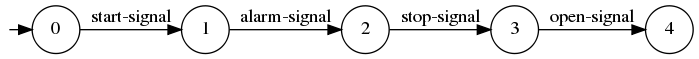
\includegraphics{src/2-framework/images/local-trace}}
\caption{LTS capturing the traces of the MSC of Fig.~\ref{image:train-scenario-all-agents} from the local point of view of the \artifact{Controller}.\label{image:local-traces-lts}}
\end{figure}

When considering traces from the perspective of the whole MSC, two interpretations co-exist. In the former, a reasoning similar to the previous one is applied. Indeed, one can consider that a MSC defines a \emph{maximal} trace, with all events in a (graphical) top-down ordering. In the example at hand, such a trace would be \artifact{<start-signal, start, alarm-pressed, \ldots, open>}. Making so amounts to consider that a MSC defines a total order among all events; this leads to a simple and straightforward, yet limited, trace semantics of MSCs.

However, when considering concurrent systems, a partial ordering among events seems more adequate~\cite{ITU:1996, Uchitel:2003}. Consider for example the events \artifact{start-signal} and \artifact{alarm-pressed} at beginning of the same MSC shown in Fig.~\ref{image:train-scenario-all-agents}. These two events model unrelated message passing between different agents, and can therefore hardly be considered timely ordered (e.g. maybe does the passenger push the alarm button when the \artifact{start-signal} is already sent but before \artifact{start} has been propagated? or even before \artifact{start-signal}?, and so on.). To take such cases into account, one has to consider that the traces defined by a MSC are \emph{linearizations} of the partial order among events. In other words, linearizations capture all possible sequences of events that respect the total ordering defined by timelines. We do not formalize the structure of Message Sequence Charts and their linearizations here, and refer the reader to~\cite{Uchitel:2003} for such a mathematical characterization. However, we state the relations that hold between the set of traces obtained with the local and global perspectives discussed so far:

\vspace{-0.4cm}
\begin{equation}
\label{equation:msc-composition}
\mathcal{L}_{total}(M) \subseteq \mathcal{L}_{partial}(M) = \mathcal{L}(M_{\downarrow Ag_1} \parallel \ldots \parallel M_{\downarrow Ag_n})
\end{equation}

The left part simply states that traces under a partial ordering certainly include those under a total ordering, which is expected. Indeed, the model with partial ordering is more general than the one with total ordering. Among others, it means that everything that is true for the former is certainly true for the latter as well. From now on, and unless stated otherwise, we therefore assume the general model with partial ordering. In particular, we do not make the $partial$ and $total$ subscripts explicit when stating other language relations in the following sections. A consistent use of one of them renders all formula valid.

The right part provides a simple way of computing all linearizations of a MSC as an (acyclic) transition system, through LTS composition. Such a LTS is illustrated in Fig.~\ref{image:msc-linearizations} for the MSC of Fig.\ref{image:train-scenario-all-agents}. As shown, the latter accepts six different linearizations, due to the possible interleaving of its first four events. By construction, such a LTS has only one initial state (the leftmost one) and only one terminating state (the rightmost one). This allows us to loosely refer to \emph{the} terminating state of an MSC (more precisely, of the LTS capturing its traces) with a precise underlying meaning.

\aside{The reader wondering whether certain linearizations are not \emph{implied} scenarios~\cite{Uchitel:2004} or whether our initial scenario should not be regarded flawed is referred to Section~\ref{section:background-discussion} where those issues are further examined.}

\begin{figure}\centering
\scalebox{0.31}{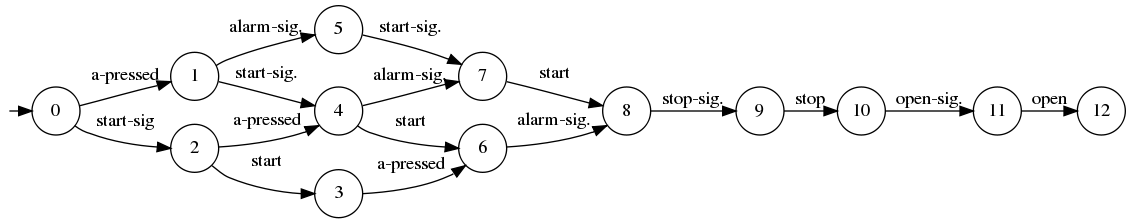
\includegraphics{src/2-framework/images/linearizations}}
\caption{LTS capturing all event linearizations of the MSC of Fig.~\ref{image:train-scenario-all-agents}. Here, \artifact{alarm-pressed} is abbreviated as \artifact{a-pressed} and \artifact{sig.} stands for \artifact{signal}. \label{image:msc-linearizations}}
\end{figure}

\subsubsection*{Multi-view model consistency}

The trace semantics of a single MSC can now be explicitly related to the notions of agent and system behaviors, also captured with LTSs in Section~\ref{section:background-agents-system-behaviors}. This amounts to define consistency rules between them, and explains the similitude between definitions \ref{equation:system-composition} and \ref{equation:msc-composition}.

Consider a system composed of $n$ agents whose behavior is modeled as $S = (Ag_1 \parallel \ldots \parallel Ag_n)$. Let $M$ denote a MSC illustrating interactions between them. We say that $M$ is \emph{consistent} with $S$ -- or, more accurately, that $M$ and $S$ \emph{are} consistent -- if the following conditions hold:

\begin{itemize}
\item $M$ and $S$ are \emph{architecturally} consistent,
\item $\mathcal{L}(M_{\downarrow Ag_i}) \subseteq \mathcal{L}(Ag_i)$ for each agent $Ag_i$, and
\item $\mathcal{L}(M) = \mathcal{L}(M_{\downarrow Ag_1} \parallel \ldots \parallel M_{\downarrow Ag_n}) \subseteq \mathcal{L}(Ag_1 \parallel \ldots \parallel Ag_n) = \mathcal{L}(S)$
\end{itemize}

The first condition is not formalized but simply requires the MSC and the system to agree on the set of agents (a MSC may actually illustrate interactions among a proper subset of system agents) and their respective interfaces (labels along a timeline are a subset of the alphabet of the corresponding agent). The second condition states that the traces defined by a timeline in the MSC must be traces accepted in the LTS modeling the behavior of the corresponding agent. The third condition states that all linearizations of the MSC must be accepted traces of the LTS modeling the behavior of the composed system. Note that, under architectural consistency, the second condition implies the third one~\cite{Uchitel:2003}. Last, but not least, stated conditions restrict consistent MSCs to those starting in the system initial state.

\subsection{Negative scenarios}

While positive MSCs model examples of behavior that the system is expected to exhibit, it is often convenient to be able to model the counterpart, that is examples of behavior that the system is expected (even required) \emph{not} to exhibit. Such proscribed behaviors are illustrated with negative MSCs~\cite{Uchitel:2004}. A negative MSC is simply a scenario whose last event is proscribed, as depicted by a crossed arrow below a dashed line. An example is given in Fig.~\ref{image:train-negative-scenario}, where the \artifact{Controller} may not open doors immediately after having started the train.

\begin{figure}[H]\centering
\scalebox{0.75}{
  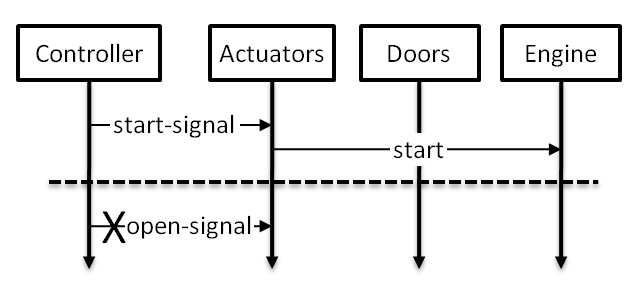
\includegraphics[trim=2mm 2mm 2mm 2mm, clip]{src/2-framework/images/train-negative-scenario}
}
\caption{A negative scenario illustrating that the controller may not open doors after having started.\label{image:train-negative-scenario}}
\end{figure}

More precisely, a negative MSC is a pair $(P,e)$ where $P$ is a positive MSC and $e$ is a single event (given our simplifying assumption, the latter event can simply be denoted by its label $l = label(e)$). The positive scenario $P$ is called the $precondition$ and $e$ the \emph{proscribed event}. The intuitive semantics is that, once the precondition has occurred from the system initial state, $e$ may not be the (very) \emph{next} event in the system. We make this semantics fully precise now. First, if the precondition of a negative MSC $N = (P,e)$ is a positive MSC, it certainly defines sets of positive traces:

\vspace{-0.2cm}
\begin{equation*}
\mathcal{L}^{+}(N) = \mathcal{L}(P)
\end{equation*}

\noindent In addition, it defines the following set of negative traces:

\vspace{-0.2cm}
\begin{equation*}
\mathcal{L}^{-}(N) = \{~w.l \mid w \in mt(\mathcal{L}(P)) \wedge l = label(e)~\}
\end{equation*}

That is, negative traces are maximal traces of the precondition concatenated with the label of the proscribed event. Note that such a definition implies that the precondition must occur completely for the proscribed event to be taken into account. In other words, partial orderings between the proscribed event and those in the precondition are never considered. This is the intended meaning of the dashed line separating them~\cite{Uchitel:2004}. 

Traces defined by a negative MSC $N = (P,e)$ can be modeled by extending the LTS modeling $\mathcal{L}_{arch}(P)$ with a new transition, labeled with $label(e)$, from its (previously) terminating state to a new error state.

\subsubsection*{Multi-view model consistency}

Similarly to positive MSCs, we state conditions for a negative MSC $N = (P,e)$ and a system $S = (Ag_1 \parallel \ldots \parallel Ag_n)$ to be consistent, as follows:

\begin{itemize}
\item $N$ and $S$ are \emph{architecturally} consistent,
\item $P$ and $S$ are consistent, and
\item $\mathcal{L}^{-}(N) \not\subseteq \mathcal{L}(Ag_1 \parallel \ldots \parallel Ag_n) = \mathcal{L}(S)$
\end{itemize}

The first condition is similar to what has been said previously for positive MSCs. The second enforces the precondition to be a consistent (positive) MSC, implicitely requiring positive traces to be accepted. The last one states that the system may not exhibit any negative trace captured by the negative MSC. Here as well, inter-consistency rules are given for the general model with partial ordering and imply consistency in the stronger model with total ordering.

\subsection{Scenario collections}

Systems are generally illustrated with multiple positive and negative scenarios. The most straightforward way of doing so is through a scenario collection $Sc = (S^+,S^-)$ where $S^+$ and $S^-$ are finite (but possibly empty) sets of positive MSCs and negative MSCs, respectively. It is straightforward, yet useful, to extend the notions of language and consistency of scenarios to collections of them. 

The positive and negative languages defined by a scenario collection $Sc = (S^+,S^-)$ are simply defined via the union on languages, but taking into account the fact that negative scenarios define positive traces in addition to negative ones:

\vspace{-0.5cm}
\begin{align*}
\mathcal{L}^+(Sc) &= \bigcup_{P \in S^+} \mathcal{L}(P)~~\cup~~\bigcup_{N \in S^{-}} \mathcal{L}^{+}(N) \\
\mathcal{L}^-(Sc) &= \bigcup_{N \in S^-} \mathcal{L}^{-}(N)
\end{align*}

Also, a scenario collection and a system are said to be consistent if and only if each positive and each negative MSC of the collection is itself consistent with the system. We extend this to the consistence of the collection of scenarios itself as follows: two sets of positive and negative scenarios, $S^+$ and $S^-$, are consistent with each other if there exists a system which is consistent with them taken as a collection $Sc = (S^+,S^-)$. A necessary condition for a scenario collection to be consistent (but not sufficient, because architectural consistency is not taken into account here) is the disjointness of positive and negative traces:

\begin{center}
$Sc = (S^+,S^-)$ is consistent only if $\mathcal{L}^+(Sc) \cap \mathcal{L}^-(Sc) = \emptyset$
\end{center}

Note that, by definition, a collection cannot be consistent with a system unless all scenarios start in its initial state. Also, since scenarios and scenario collections are both finite, a collection is hardly complete in practice because most systems accept an infinite number of traces, through loops. Last, the fact that all scenarios must start in the same initial state may imply a lot of redundancy in descriptions of large systems. Among others, this can render consistency difficult to guarantee unless costly refactoring steps are conducted on scenarios. High-level Message Sequence Charts (hMSCs), introduced in the next section, provide a mean to tackle these problems.

\subsection[Flowcharting scenarios in high-level MSCs]{Flowcharting scenarios in high-level Message Sequence Charts\label{section:background-hmsc}}

A High Level Message Sequence Chart is a directed graph where each node refers to a MSC (named \emph{basic} MSC, bMSC for short) or a finer grained hMSC~\cite{ITU:1996}. We ignore this later possibility until further notice. Outgoing edges of a node capture its possible continuations, allowing the user to introduce sequences, alternatives and loops, to reuse small MSC fragments, and so on. An hMSC also has an initial starting point that indicates the initial system state. An example of hMSC is given in Fig.~\ref{image:train-hmsc}. 

\vspace{0.4cm}
\begin{figure}[H]\centering
\scalebox{0.66}{
  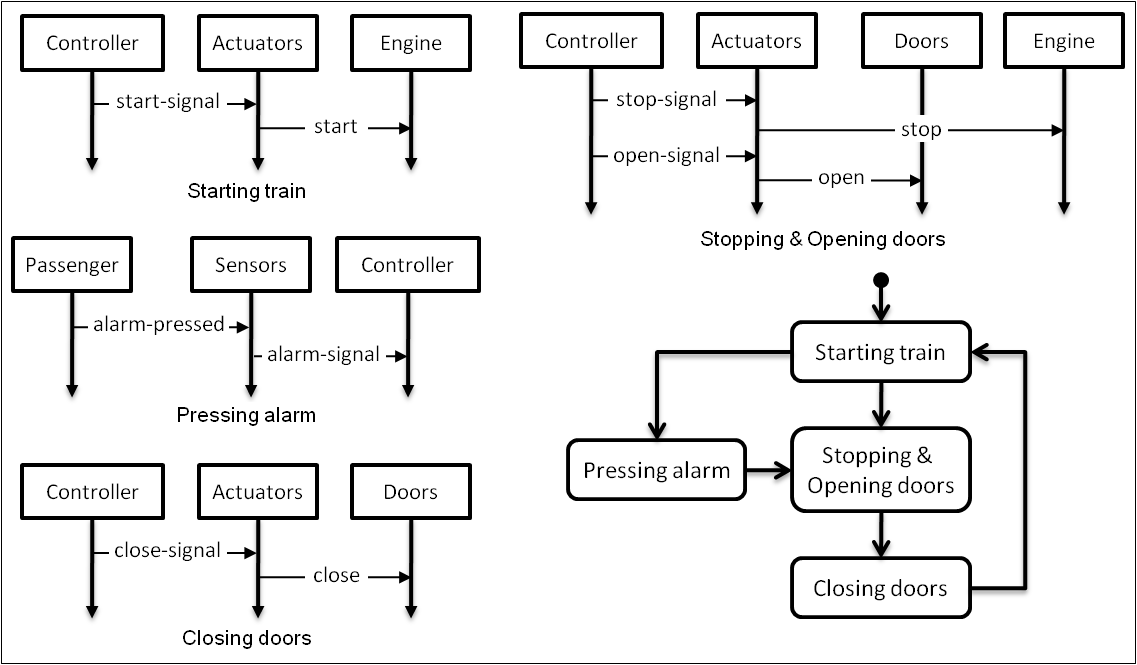
\includegraphics[trim=2mm 2mm 2mm 2mm, clip]{src/2-framework/images/train-hmsc}
}
\caption{A high-level Message Sequence Chart for the train system.\label{image:train-hmsc}}
\end{figure}

A trace semantics can of course be given to hMSCs, which amounts to answering the question \emph{what traces are captured by a hMSC?} This apparently simple question has, however, a more complex answer. The reasons are actually manifold; we summarize here, and slightly extend, the characterization given in~\cite{Uchitel:2004}.

First of all, some hMSCs do not define regular languages~\cite{Henriksen:2000}, and therefore have sets of traces that cannot be modeled with LTS. Therefore, we must restrict our framework to regular hMSCs. Under total ordering of events inside bMSCs, hMSCs are regular. Under partial ordering, a sufficient condition for being regular is that the hMSC does not contain a cycle in which two disjoint sets of agents interact independently of each other. We assume such \emph{bounded} hMSCs in the sequel. 

Also, in addition to the partial or total ordering of events in bMSCs, two interpretations co-exist about how a system evolves from a bMSC to another inside a hMSC. The first one, called \emph{strong sequential composition}, is to assume that all agents wait until all events of a bMSC have occurred before moving on to the next one. This implies that there is an implicit synchronisation scheme used by agents to know when a scenario has been completed. The other one, \emph{weak sequential composition}, does not make such an assumption and allows an agent to move from a bMSC to another one without having to synchronize with the other agents. Given the independence between assumptions of partial/total event ordering and weak/strong sequential composition, four combinations actually exist. To keep things simple enough, and because they lead to strange concurrency models\footnote{in particular, one can check that such models are very sentitive to bMSC concatenation and decomposition}, we do not consider partial (resp. total) ordering with strong (resp. weak) sequential composition. In the sequel, therefore, strong (resp. weak) sequential composition implies total ordering (resp. partial) of MSC events.

Under these assumptions, the trace analysis for hMSCs is very similar to what has been done for MSCs, and therefore leads to language relations similar to the ones given for the latter in Section~\ref{subsection:background-positive-scenarios} (see equation~\ref{equation:msc-composition}):

\begin{equation}
\mathcal{L}_{strong}(H) \subseteq \mathcal{L}_{weak}(H) \subseteq \mathcal{L}(H_{\downarrow Ag_1} \parallel \ldots \parallel H_{\downarrow Ag_n})
\label{equation:hsmc-traces-by-agent-composition}
\end{equation}

The set of traces $\mathcal{L}_{strong}(H)$ and $\mathcal{L}_{weak}(H)$ are easily explained by considering scenarios ``built'' by the hMSC. Consider a finite path in the hMSC. Concatenating the bMSCs along this path ``builds'' a single MSC. For example, concatenating \artifact{Starting train}, \artifact{Pressing alarm} and \artifact{Stopping \& Opening the doors} in the hMSC of Fig.~\ref{image:train-hmsc} leads to the MSC of Fig.~\ref{image:train-scenario-all-agents}. From results in Section~\ref{subsection:background-positive-scenarios}, such a MSC $M$ defines the set of traces $\mathcal{L}_{total}(M)$ and $\mathcal{L}_{partial}(M)$. To define traces defines by a hMSC $H$, we have to consider all such possible MSCs: 

\vspace{-0.5cm}
\begin{align*}
\mathcal{L}_{strong}(H) &= \bigcup_{M \in H} \mathcal{L}_{total}(M) \\
\mathcal{L}_{weak}(H) &= \bigcup_{M \in H} \mathcal{L}_{partial}(M)
\end{align*}

%\vspace{-0.8cm}
\noindent where $M \in H$ means ``the MSC $M$ can be built by $H$'', with the obvious meaning in terms of possible paths in $H$. The language $\mathcal{L}_{weak}$ corresponds to the notion of \emph{trace model} in~\cite{Uchitel:2004}.

Now, one can actually consider another way to compute the set of traces defined by a hMSC. In this alternative way, the local perspective of the agent timelines is taken into account, in a way similar to what has been done for MSCs. This leads to the rightmost part of the relations between hMSC languages in~\ref{equation:hsmc-traces-by-agent-composition}, that computes hMSC traces as the composition of local agent traces $H_{\downarrow Ag_i}$. The composition of such a LTS for each agent correspond to the notion of \emph{minimal architecture model} in~\cite{Uchitel:2004} and will sometimes be denoted by $\mathcal{L}_{arch}(H)$.

An algorithm can be found in~\cite{Uchitel:2004} for synthesizing the LTS modeling $\mathcal{L}_{arch}(H)$. For a given agent $Ag_{i}$, the LTS $H_{\downarrow Ag_i}$ is synthesized by connecting the LTSs $M_{\downarrow Ag_i}$ corresponding to each bMSC $M$ with $\tau$ transitions, according to their possible continuations given by hMSC edges. This construction is illustrated in Fig.~\ref{image:XX} for the hMSC of Fig.~\ref{image:train-hmsc} and the \artifact{Controller} agent. The resulting LTS can be further simplified by removing $\tau$ transitions and minimizing the LTS.  Note that, thanks to the simplicity of the model with strong sequential composition, $\mathcal{L}_{strong}(H)$ can be computed in a very similar way. In contrast, $\mathcal{L}_{weak}(H)$ is much harder to model as a LTS; a synthesis algorithm can however be found in~\cite{Uchitel:2004}.

\aside{One can note an important difference between the relations between MSC languages in~\ref{equation:msc-composition} and those between hMSC languages in~\ref{equation:hsmc-traces-by-agent-composition}. Indeed, the former denotes an equality between $\mathcal{L}_{partial}(M)$ and $\mathcal{L}(M_{\downarrow Ag_1}\parallel\ldots\parallel M_{\downarrow Ag_n})$ while the latter defines a set inclusion between $\mathcal{L}_{weak}(H)$ and $\mathcal{L}(H_{\downarrow Ag_1}\parallel\ldots\parallel H_{\downarrow Ag_n})$. In fact, traces in $\mathcal{L}_{arch}(H) \setminus \mathcal{L}_{weak}(H)$ capture the set of \emph{implied} scenarios of a hMSC specification~\cite{Alur:2000, Uchitel:2004}. Implied scenarios occur when a system is designed globally (the hMSC) while implemented component-wise (the composition of agent LTSs). In other words, implied scenarios capture traces that follow different paths in the hMSC when projected on individual agent timelines. We come back to them in Section~\ref{section:background-discussion}.}

\subsubsection*{Finer-grained hMSC}

As stated previously, a hMSC node can refer to a finer-grained hMSC instead of a bMSC. Taken them into account in the trace semantics given previously requires deciding how a sub-hMSC has to be ``connected'' with its father. To keep a consistent framework in terms of synchronization hypotheses, we require such a sub-hMSC to have, in addition to its initial state, a terminating state to which at least one node is connected. For simplicity, we also forbid nodes with no outgoing transition. Under such assumptions, it is relatively easy to ``unfold'' a hMSC as another one with all nodes refined as basic MSCs. The trace semantics remains unchanged and is defined in terms of the latter ``flat'' hMSC. 

In practice, this flat hMSC must not be explicitely constructed when synthesizing the LTS for $\mathcal{L}_{arch}$. Indeed, the LTSs $H_{\downarrow Ag_i}$ of finer-grained hMSCs respecting our constraints present only one initial state and only one terminating state, allowing them to be connected with $\tau$ transitions in the same way than LTSs $M_{\downarrow Ag_i}$. Similar argument applies for $\mathcal{L}_{strong}$, but not for $\mathcal{L}_{weak}$.

\subsubsection*{Multi-view model consistency}
 
Based on the trace semantics defined in the previous section, we can now define additional consistency rules in our framework. We say that a hMSC $H$ and a system $S = (Ag_1 \parallel \ldots \parallel Ag_n)$ are consistent if the following condition holds:

\begin{itemize}
\item $H$ and $S$ are \emph{architecturally} consistent,
\item $\mathcal{L}(H_{\downarrow Ag_i}) \subseteq \mathcal{L}(Ag_i)$ for each agent $Ag_i$, and
\item $\mathcal{L}_{arch}(H) = \mathcal{L}(H_{\downarrow Ag_1} \parallel \ldots \parallel H_{\downarrow Ag_n}) \subseteq \mathcal{L}(Ag_1 \parallel \ldots \parallel Ag_n) = \mathcal{L}(S)$
\end{itemize}

These conditions are the counterpart of those given previously for MSCs and have a similar interpretation, \emph{mutatis mutandis}. In addition, however, it is convenient to distinguish between a hMSC that describes all behaviors of a system and one that only illustrates a subset of them. This leads to the notion of hMSC completeness. A hMSC $H$ is \emph{complete} for a system $S = (Ag_1 \parallel \ldots \parallel Ag_n)$ if it is consistent with it and defines the same language, that is, if $\mathcal{L}_{arch}(H) = \mathcal{L}(S).$


\section{State-based invariants through Fluents}

\subsection{Decorating LTS with invariants}

\section{Declarative goals and domain properties}

\section{Discussion\label{section:background-discussion}}
